% -- Generated using the code: resting_clocks_single_fig(0, 6, 0.5)



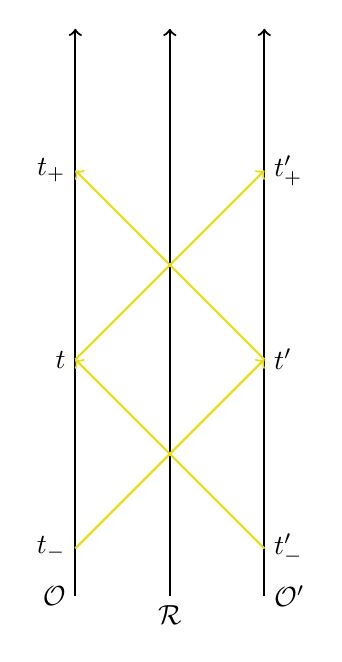
\begin{tikzpicture}[scale=1.2]
	% Draw lines of observers
	\draw[->, thick] (-1.0, 0) -- (-1.0, 6);
	\draw[->, thick] (1.0, 0) -- (1.0, 6);
	\draw[->, thick] (0.0, 0) -- (0.0, 6);
	
	% Draw trajectories of light
	\draw[->, thick, black!10!yellow] (-1.0, 0.5) -- (1.0, 2.5);
	\draw[->, thick, black!10!yellow] (1.0, 2.5) -- (-1.0, 4.5);
	\draw[->, thick, black!10!yellow] (1.0, 0.5) -- (-1.0, 2.5);
	\draw[->, thick, black!10!yellow] (-1.0, 2.5) -- (1.0, 4.5);
	
	% Make labels
	\draw (-1.0, 0) node[left] {$\mathcal{O}$};
	\draw (-1.0, 0.5) node[left] {$t_-$};
	\draw (-1.0, 4.5) node[left] {$t_+$};
	\draw (1.0, 2.5) node[right] {$t'$};
	\draw (1.0, 0) node[right] {$\mathcal{O}'$};
	\draw (1.0, 0.5) node[right] {$t'_-$};
	\draw (1.0, 4.5) node[right] {$t'_+$};
	\draw (-1.0, 2.5) node[left] {$t$};
	\draw (0.0, 0) node[below] {$\mathcal{R}$};
\end{tikzpicture}